% Options for packages loaded elsewhere
\PassOptionsToPackage{unicode}{hyperref}
\PassOptionsToPackage{hyphens}{url}
%
\documentclass[
]{book}
\usepackage{lmodern}
\usepackage{amssymb,amsmath}
\usepackage{ifxetex,ifluatex}
\ifnum 0\ifxetex 1\fi\ifluatex 1\fi=0 % if pdftex
  \usepackage[T1]{fontenc}
  \usepackage[utf8]{inputenc}
  \usepackage{textcomp} % provide euro and other symbols
\else % if luatex or xetex
  \usepackage{unicode-math}
  \defaultfontfeatures{Scale=MatchLowercase}
  \defaultfontfeatures[\rmfamily]{Ligatures=TeX,Scale=1}
\fi
% Use upquote if available, for straight quotes in verbatim environments
\IfFileExists{upquote.sty}{\usepackage{upquote}}{}
\IfFileExists{microtype.sty}{% use microtype if available
  \usepackage[]{microtype}
  \UseMicrotypeSet[protrusion]{basicmath} % disable protrusion for tt fonts
}{}
\makeatletter
\@ifundefined{KOMAClassName}{% if non-KOMA class
  \IfFileExists{parskip.sty}{%
    \usepackage{parskip}
  }{% else
    \setlength{\parindent}{0pt}
    \setlength{\parskip}{6pt plus 2pt minus 1pt}}
}{% if KOMA class
  \KOMAoptions{parskip=half}}
\makeatother
\usepackage{xcolor}
\IfFileExists{xurl.sty}{\usepackage{xurl}}{} % add URL line breaks if available
\IfFileExists{bookmark.sty}{\usepackage{bookmark}}{\usepackage{hyperref}}
\hypersetup{
  pdftitle={Manuel utilisateur Hypothesis},
  pdfauthor={Jean-Marc Meunier},
  hidelinks,
  pdfcreator={LaTeX via pandoc}}
\urlstyle{same} % disable monospaced font for URLs
\usepackage{longtable,booktabs}
% Correct order of tables after \paragraph or \subparagraph
\usepackage{etoolbox}
\makeatletter
\patchcmd\longtable{\par}{\if@noskipsec\mbox{}\fi\par}{}{}
\makeatother
% Allow footnotes in longtable head/foot
\IfFileExists{footnotehyper.sty}{\usepackage{footnotehyper}}{\usepackage{footnote}}
\makesavenoteenv{longtable}
\usepackage{graphicx,grffile}
\makeatletter
\def\maxwidth{\ifdim\Gin@nat@width>\linewidth\linewidth\else\Gin@nat@width\fi}
\def\maxheight{\ifdim\Gin@nat@height>\textheight\textheight\else\Gin@nat@height\fi}
\makeatother
% Scale images if necessary, so that they will not overflow the page
% margins by default, and it is still possible to overwrite the defaults
% using explicit options in \includegraphics[width, height, ...]{}
\setkeys{Gin}{width=\maxwidth,height=\maxheight,keepaspectratio}
% Set default figure placement to htbp
\makeatletter
\def\fps@figure{htbp}
\makeatother
\setlength{\emergencystretch}{3em} % prevent overfull lines
\providecommand{\tightlist}{%
  \setlength{\itemsep}{0pt}\setlength{\parskip}{0pt}}
\setcounter{secnumdepth}{5}
\usepackage{booktabs}
\usepackage[]{natbib}
\bibliographystyle{apalike}

\title{Manuel utilisateur Hypothesis}
\author{Jean-Marc Meunier}
\date{2020-10-06}

\begin{document}
\maketitle

{
\setcounter{tocdepth}{1}
\tableofcontents
}
\hypertarget{section}{%
\chapter*{\texorpdfstring{\protect
\includegraphics{img/hypothesislogomark.png}}{}}\label{section}}
\addcontentsline{toc}{chapter}{}

Ce manuel propose une synthèse en français des \href{https://web.hypothes.is/help-categories/tutorials/}{tutoriels pour hypothesis}. Je l'ai rédigé pour les étudiants de l'institut d'enseignement à distance de \href{https://www.univ-paris8.fr/}{l'université Paris 8}. Il est mis à disposition sous \href{https://creativecommons.org/licenses/by-nc-sa/3.0/fr/}{licence creative commons CC BY-NC-SA}.

Des remarques, des coquilles ? Utilisez \href{https://hyp.is/go?url=https\%3A\%2F\%2Fjmeunierp8.github.io\%2FGuide-utilisateur-Hypothesis\%2F\&group=__world__}{ce fil d'annotation} pour les signaler.

\hypertarget{a-quoi-uxe7a-sert}{%
\section*{A quoi ça sert ?}\label{a-quoi-uxe7a-sert}}
\addcontentsline{toc}{section}{A quoi ça sert ?}

\href{https://web.hypothes.is/}{Hypothesis} fournit un ensemble de composants qui fonctionnent ensemble pour permettre un large éventail d'applications basées sur l'annotation. ces composants sont :

\begin{itemize}
\tightlist
\item
  Un visualiseur et un éditeur d'annotations qui s'exécutent en superposition au document dans un navigateur soit grâce à une extension pour le navigateur Google Chrome, soit à l'aide d'un marque-page (bookmarklet).
\item
  Un service qui stocke, recherche et affiche les annotations, gère les utilisateurs et les groupes, et fournit le client dans des pages qui ont été annotées.
\end{itemize}

\begin{figure}
\centering
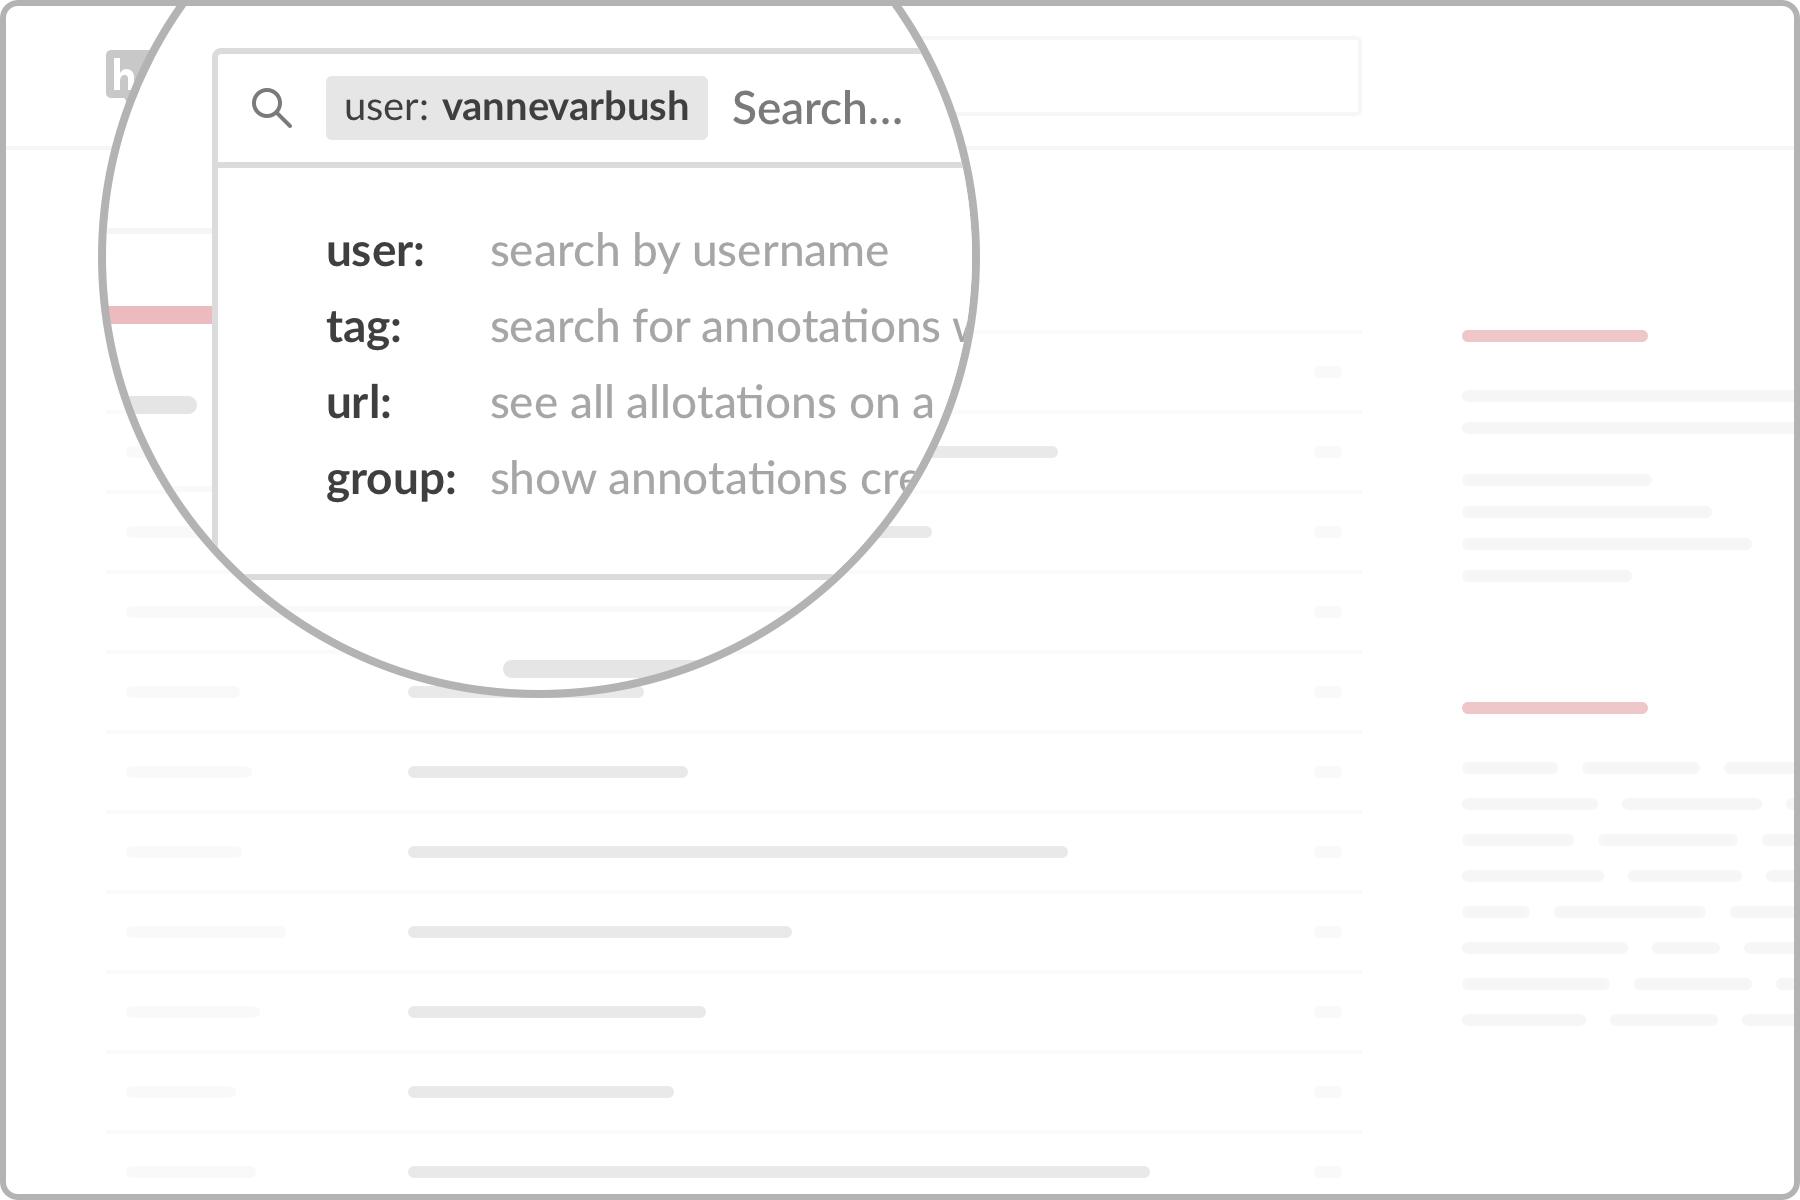
\includegraphics{img/05@2x.png}
\caption{Comment ça marche ?}
\end{figure}

\begin{itemize}
\tightlist
\item
  Une fois hypothesis installé, il suffit de sélectionnez le texte à annoter puis d'ajouter vos commentaires ou des mot-clés (tags) avant de publier publiquement ou non vos annotations.
\item
  Vous pouvez partager vos annotations à l'aide d'un lien vers une annotation ou une page. vous pouvez également répondre à toute annotation.
\item
  Hypothesis permet aussi collaborer en privé avec d'autres personnes en créant un groupe et en partageant vos annotations dans celui-ci.
\item
  Enfin, vous pouvez explorez toutes les annotations publiques et les profils.
\end{itemize}

Voici quelques ressources en anglais pour vous faire une idée des possibilités offertes par Hypothesis :

\hypertarget{pour-les-enseignants}{%
\subsection*{Pour les enseignants}\label{pour-les-enseignants}}
\addcontentsline{toc}{subsection}{Pour les enseignants}

\begin{itemize}
\tightlist
\item
  Voyez ce que les \href{https://web.hypothes.is/teacher-testimonials/}{enseignants} et les \href{https://web.hypothes.is/student-testimonials/}{étudiants} disent du l'intérêt de l'annotation collaborative
\item
  Explorer des \href{https://web.hypothes.is/examples-of-classroom-use/}{exemples d'utilisation en classe}
\item
  \href{https://web.hypothes.is/blog/back-to-school-with-annotation-10-ways-to-annotate-with-students/}{10 façons d'annoter avec les étudiants}
\item
  \href{https://web.hypothes.is/teacher-resource-guide/}{Guide pour les enseignants}
\end{itemize}

\hypertarget{pour-les-uxe9tudiants}{%
\subsection*{Pour les étudiants}\label{pour-les-uxe9tudiants}}
\addcontentsline{toc}{subsection}{Pour les étudiants}

\begin{itemize}
\tightlist
\item
  \href{https://web.hypothes.is/annotation-tips-for-students/}{Conseils d'annotation pour les étudiants}
\item
  \href{https://web.hypothes.is/student-resource-guide/}{Guide pour les étudiants}
\end{itemize}

\hypertarget{s1}{%
\chapter{Créez votre compte}\label{s1}}

Allez à la \href{https://hypothes.is/signup}{page d'inscription}. Pour créer un compte Hypothesis, il vous suffit de disposer d'une adresse électronique et d'un nom d'utilisateur. Vous devriez recevoir un courriel de confirmation. Sinon, vérifiez votre boîte à spam.

\begin{figure}
\centering
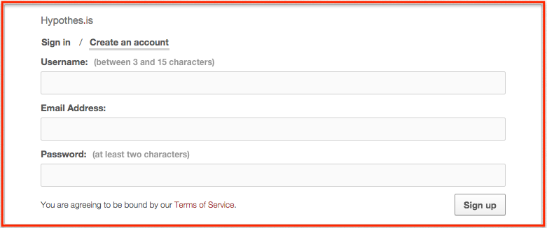
\includegraphics{img/08a7089161c6c5bd7205aa71e717ab6e.png}
\caption{Créer un compte}
\end{figure}

Vous devez ensuite \protect\hyperlink{s2}{installer hypothesis} dans votre navigateur.

\hypertarget{s2}{%
\chapter{Ajouter Hypothesis à votre navigateur}\label{s2}}

Vous devez installer l'extension Chrome ou ajouter le marque-page à votre navigateur préféré. Vous avez trois possibilités~:

\begin{itemize}
\tightlist
\item
  Vous utilisez Chrome, \protect\hyperlink{s21}{installez l'extension}
\item
  Vous utilisez un autre navigateur, \protect\hyperlink{s22}{installez le signet}
\item
  Ni l'un ni l'autre ne marche, \protect\hyperlink{s23}{collez le lien sur via.hypothesis}
\end{itemize}

\hypertarget{s21}{%
\section{Installer l'extension Chrome}\label{s21}}

Lorsque vous utilisez Google Chrome, suivez \href{https://chrome.google.com/webstore/detail/hypothesis-web-pdf-annota/bjfhmglciegochdpefhhlphglcehbmek}{ce lien vers l'extension Hypothesis dans la boutique en ligne de Chrome}. Cliquez sur ``\textbf{AJOUTER A CHROME}'' :

\begin{figure}
\centering
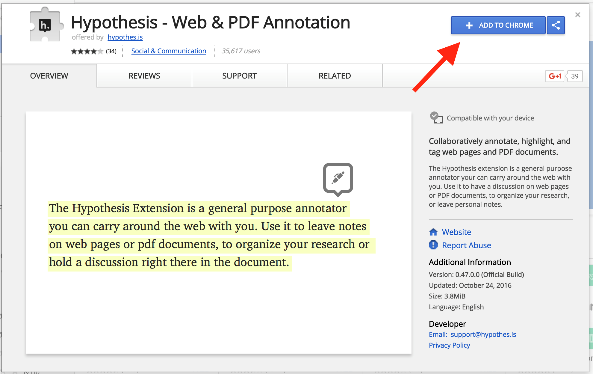
\includegraphics{img/94d5e4f1e0139b6a3709c5bfecad0737.png}
\caption{Installer l'extension}
\end{figure}

\hypertarget{s22}{%
\section{Installer le signet}\label{s22}}

Pour ceux qui utilisent Firefox, Safari ou d'autres navigateurs, le signet fournit un moyen facile d'utiliser Hypothesis dans le navigateur de votre choix. (Rappel : Si votre navigateur préféré est Chrome, veuillez consulter ces instructions pour \protect\hyperlink{s21}{installer l'extension Chrome}).

\begin{itemize}
\tightlist
\item
  Pour installer le signet Hypothesis, ouvrez le navigateur de votre choix et allez sur \href{https://web.hypothes.is/start/}{web.hypothes.is/start/}.
\item
  Sur le côté droit, vous verrez un bouton ``Hypothesis Bookmarklet''.
\item
  Glissez et déposez le bouton dans votre barre de signets, ou cliquez sur le bouton droit et sélectionnez ``\emph{bookmark this link}'' dans le menu contextuel.
\end{itemize}

\begin{figure}
\centering
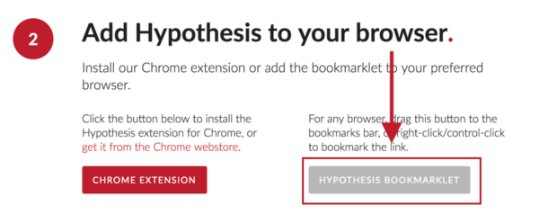
\includegraphics{img/10bf5d0ce6574ed9cbaa1f7df259038a.png}
\caption{Installer le signet}
\end{figure}

\hypertarget{s23}{%
\section{Coller un lien sur via.hypothesis}\label{s23}}

Cette option est à utiliser lorsque l'extension ou le signet ne fonctionne pas ou que vous n'avez pas la possibiité de les installer.

\begin{itemize}
\tightlist
\item
  Copiez le lien de la page à annoter
\item
  Cliquez sur le lien \url{https://via.hypothes.is/}
\item
  Collez votre lien et cliquez sur go.
\end{itemize}

Note : Vous retrouverez ce lien sur n'importe que page du site \href{https://web.hypothes.is/}{hypothesis} en cliquant en haut à droite sur \href{https://via.hypothes.is/}{Paste a link}.

\begin{figure}
\centering
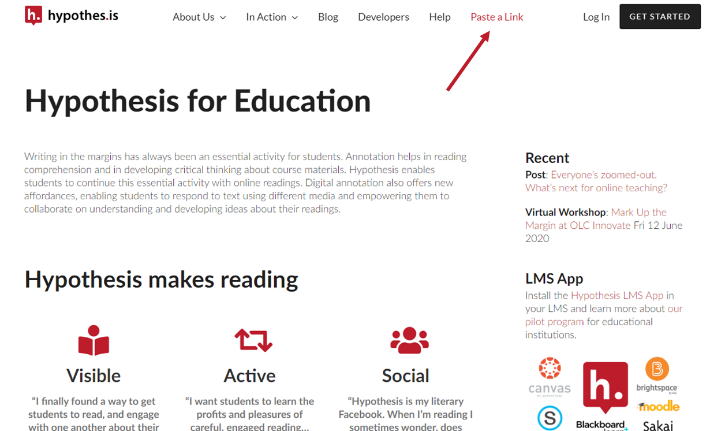
\includegraphics{img/31f63f99822907f0d22ec643cca557dd.png}
\caption{Paste a link}
\end{figure}

\hypertarget{s3}{%
\chapter{Annoter un document}\label{s3}}

Pour annoter un document, vous devez~:

\begin{itemize}
\tightlist
\item
  Accédez à n'importe quelle page web (ou fichier PDF ou EPUB dans votre navigateur)
\item
  Activez hypothesis en cliquant sur le bouton de l'extension (Chrome), le signet (autres navigateur) ou en collant le lien dans via hypothesis
\item
  Ouvrez le volet hypothesis et si ce n'est pas encore fait, connectez-vous à votre compte.
\end{itemize}

\begin{figure}
\centering
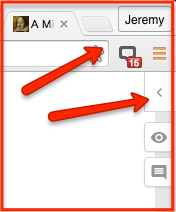
\includegraphics{img/ae9a3a75e6c3a239c6fede86ebe4fa7d.png}
\caption{Ouvrir hypothesis}
\end{figure}

\begin{itemize}
\tightlist
\item
  Sélectionnez du texte et annotez. Pour cela, vous devez saisir votre commentaire dans le champ texte. Vous disposez de quelques boutons de mise en forme et pouvez ajouter des liens, des images ou des formules mathématiques\footnote{Les formules doivent respecter la syntaxe Latex. Si vous ne la connaissez pas, utilisez ce site pour écrire votre formule~: \url{https://www.codecogs.com/latex/eqneditor.php} puis coller le code dans votre annotation entre deux symboles /\$}.
\item
  Vous pouvez également ajouter des mots-clés en les saisissant dans le champ «~Add tags~»
\end{itemize}

Vous devez ensuite valider votre annotation. Pour cela cliquez sur le bouton noir sous les mots-clés, puis sélectionnez le mode de publication~: privé (Post to me) ou public (Post to public). Si vous travaillez dans un groupe, vous pouvez également publier l'annotation pour le groupe. Le menu vous proposera alors une option Post to «~\emph{nom-du-groupe~}».

\begin{figure}
\centering
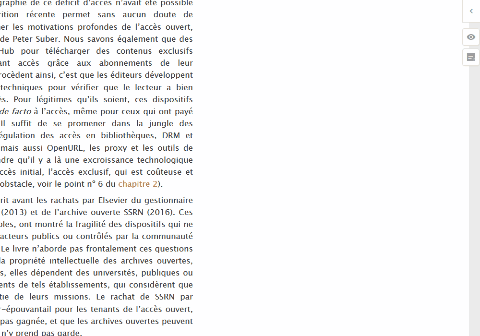
\includegraphics{img/img-5.png}
\caption{Comment annoter (Source : \href{http://www.maisondesrevues.org/1182}{La maison des revues(2019)})}
\end{figure}

'`

\hypertarget{s31}{%
\section{Conseils pour bien annoter}\label{s31}}

Voici cinq bonnes pratiques à avoir en têtes lorsque vous annotez.

\begin{enumerate}
\def\labelenumi{\arabic{enumi}.}
\item
  \textbf{Sélectionnez avec soin le texte pour vos annotations} Cela parait une évidence, mais il est bon de le rappeler et surtout de préciser ce que cela veut dire. Le choix de passages à annoter dépend principalement de l'objectif de votre lecture et de vos connaissances antérieures. Ce choix se portera sur les passages difficiles, ceux qui paraissent particulièrement important pour comprendre la progression du discours de l'auteur ou qui vont alimenter votre réflexion sur un sujet particulier. Dans tout les cas privilégiez la sélection d'un passage qui constitue une unité de sens. Lorsque vous exploiterez les annotations, il sera plus facile de renconnaitre de quoi il s'agit. Si un passage est déjà sélectionné, vous pouvez soit répondre à son annotation, soit sélectionner à nouveau le même texte. Vous pouvez également sélectionner un texte qui se trouve dans ou qui comporte une autre mise en évidence ou une autre annotation. Le choix n'est pas anodin à la fois pour la lisibilité des annotations, mais aussi pour la communication vers les autres usagers.
\item
  \textbf{Une annotation doit ajouter quelque chose au texte.} Les annotations servent la plupart du temps de support à l'analyse et pas simplement au résumé du texte. Elles sont la marque de votre travail de réflexion et d'apprentissage. L'annotation peut ainsi ajoter une définition, un lien vers un autre document, une autre idée. Ce peut également être un codage des différentes partie du texte ou du passage que vous annotez. Ce que vous ajouterez dépend bien sûr de l'objectif de votre lecture. Ainsi lors de la lecture du texte d'un cours, les annotations peuvent tout simplement être les questions à poser à l'enseignant.
\item
  \textbf{Utiliser la mise en forme des annotations.} Lorsqu'on doit manipuler des textes longs, surtout s'ils sont enrichis d'annotations, utiliser des repères visuels peut s'avérer particulièment important. N'hésitez pas à faire usage des possiblités de mise en forme de vos annotations et d'utiliser les listes à puces pour facililter la lecture ultérieure.
\item
  \textbf{Utilisez des liens et des images.} Comme avec les possibilités de mise en forme, ces fonctionnalités sont particulièrement importantes pour aider à lexploration des annotations. Elles permettent en outre de faire des connexions avec d'autres documents et ainsi d'enrichir votre document.
\item
  \textbf{Utilisez des mots-clés}. Votre professeur peut vous demander d'utiliser des étiquettes pour diverses raisons. Un hashtag de cours peut être particulièrement utile car il génère un flux de contenu lié au tag sur le site Hypothesis. Cela vous permettra, à vous et à vos camarades de classe, de suivre plus facilement le travail des autres. Un enseignant peut vous demander d'identifier certains éléments textuels. Les mots-clés peuvent également être utiles pour vous même. pour faciliter la collecte d'arguments en faveur d'une thèse et des citations à utiliser dans un document final.
\end{enumerate}

\hypertarget{s4}{%
\chapter{Partager les annotations}\label{s4}}

Chaque élément dans hypothesis possède sa propre URL et peut ainsi être partagé.

\hypertarget{s41}{%
\section{Partager un fil d'annotation}\label{s41}}

Vous pouvez partager toutes les annotations d'une page web ou d'un document. Pour cela ouvrez le volet d'annotation et cliquez sur l'icone 
\includegraphics{img/9ed8e6410bcd25e02923bf774a7fb2fe.png} en haut à droite du volet. Vous aurez ainsi accès au lien de partage de la page qu'il vous suffira d'envoyer à votre correspondant.

\begin{figure}
\centering
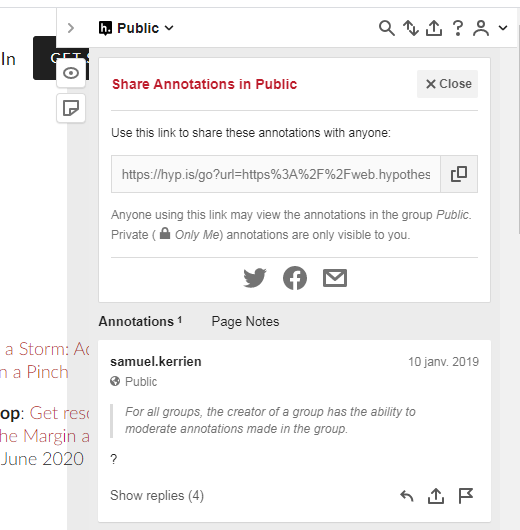
\includegraphics{img/cdbebac10f9bd02f38ed117c1ab8e322.png}
\caption{Partager un fil d'annotations}
\end{figure}

\hypertarget{s42}{%
\section{Partager une annotation}\label{s42}}

Vous pouvez ne partager qu'une annotation ou une réponse à une annotation. Après l'avoir repérée dans le fil d'annotation (voir la \protect\hyperlink{s7}{section 7}), cliquez sur le lien de partage sous l'annotation 
\includegraphics{img/9ed8e6410bcd25e02923bf774a7fb2fe.png}, puis comme précédemment copiez le lien et envoyez-le.

\begin{figure}
\centering
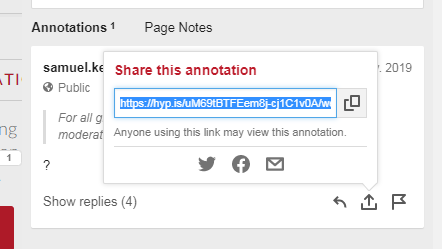
\includegraphics{img/cb6bdc80ca52dfbde7f2cb85ae981643.png}
\caption{Partager une annotation}
\end{figure}

\hypertarget{s5}{%
\chapter{Modification ou suppression d'une annotation}\label{s5}}

Sous chaque annotation vous avez un bouton en forme de crayon vous permettant de modifier celle-ci et un autre en forme de poubelle pour la supprimer.

\begin{figure}
\centering
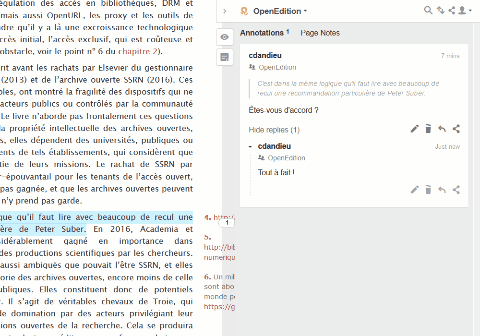
\includegraphics{img/523575cc7eaccc9577140afd392b9710.png}
\caption{Modifier ou supprimer une annotation (Source : \href{http://www.maisondesrevues.org/1182}{La maison des revues(2019)})}
\end{figure}

\hypertarget{s6}{%
\chapter{Travailler en groupe avec hypothesis}\label{s6}}

Sous hypothesis, un groupe est un ensemble de documents et d'annotations réservés aux seuls utilisateurs invités par le créateur du groupe.

\hypertarget{s61}{%
\section{Créer à un groupe}\label{s61}}

Pour créer un groupe, ouvrez le volet d'annotation puis déroulez le menu des groupes. Sélectionnez alors le groupe de votre choix ou cliquez sur \emph{«~New private group~»} pour en créer un nouveau.

\begin{figure}
\centering
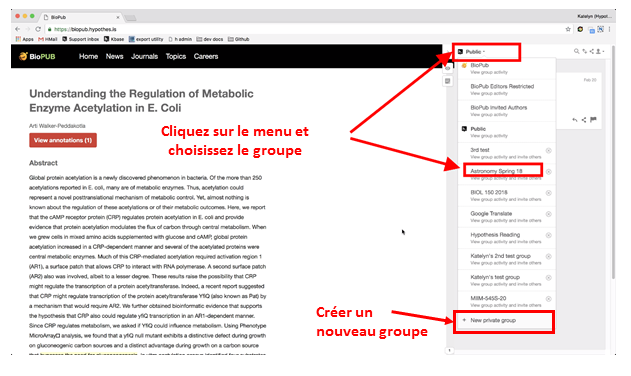
\includegraphics{img/groupes.png}
\caption{consulter ou créer un groupe}
\end{figure}

\hypertarget{s62}{%
\section{Inviter d'autres personnes dans un groupe}\label{s62}}

Pour inviter quelqu'un à rejoindre votre groupe, vous devez lui envoyer le lien de connexion.
* Ouvrez le menu des groupes, puis repérez votre groupe.
* Cliquez sur le chevron à droite du nom, puis cliquez sur \emph{«~Copy invite link~»}
* Envoyez ce lien à la personne que vous voulez inviter.

\begin{figure}
\centering
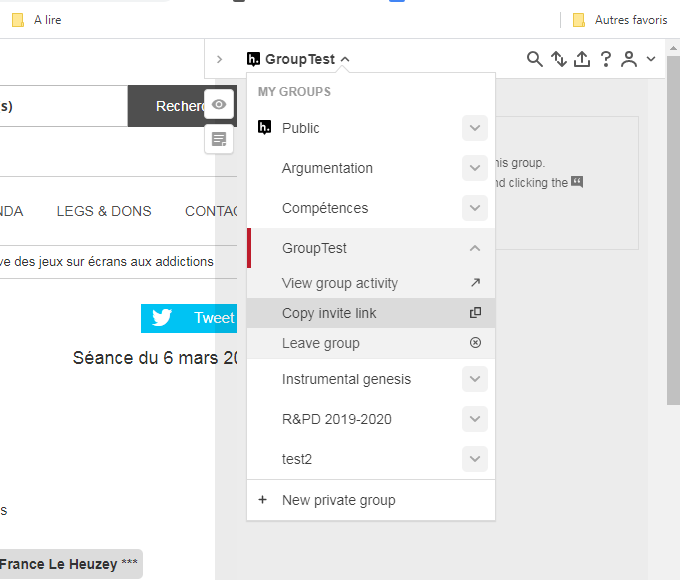
\includegraphics{img/10545b5bdaaf92692913d7f2ab400691.png}
\caption{Inviter à rejoindre un groupe}
\end{figure}

\hypertarget{s63}{%
\section{Rejoindre un groupe}\label{s63}}

Pour rejoindre un groupe, il faut qu'un membre vous invite en vous envoyant lien. Après vous être connecté à votre compte, cliquez sur le bouton pour faire partie du groupe.

\begin{figure}
\centering
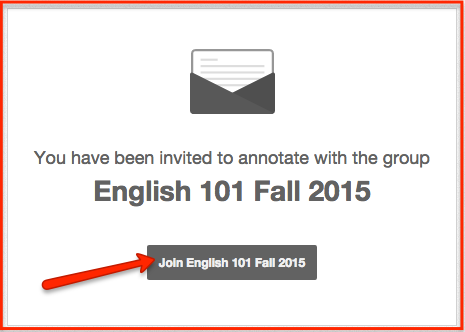
\includegraphics{img/3c43f5853bd5bc770efb60d74686f1ae.png}
\caption{Rejoindre un groupe}
\end{figure}

\hypertarget{s64}{%
\section{Annoter un document dans un groupe}\label{s64}}

Lorsque vous annotez un document dans un groupe, vous pouvez faire des annotations uniquement pour vous-même en sélectionnant l'option «~Only me~» dans le bouton de validation ou pour tous les membres du groupe en sélectionnant le nom du groupe.

\begin{figure}
\centering
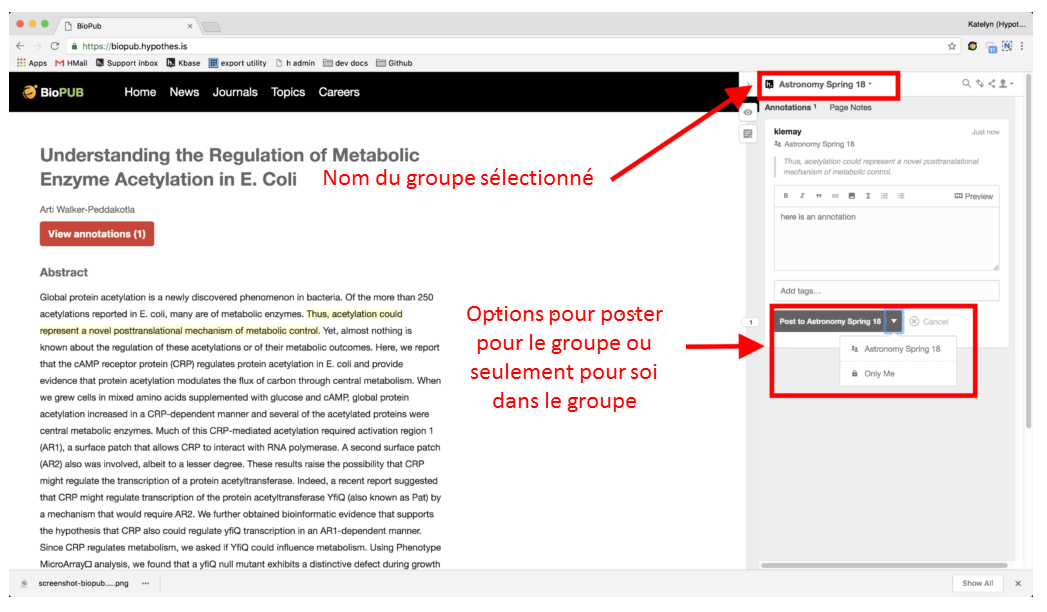
\includegraphics{img/postGroup.png}
\caption{Poster une annotation dans un groupe}
\end{figure}

\hypertarget{s65}{%
\section{Répondre à une annotation}\label{s65}}

Dans un certain nombre de cas, vous pouvez avoir à répondre à une annotation. Dans ce cas, ouvrez le document sous hypothesis et cherchez l'annotation (voir \protect\hyperlink{s7}{section 7}, puis cliquez sur la flèche sous l'annotation à laquelle vous voulez répondre, saisissez votre réponse et validez-la (Clic sur «~Post to~\ldots)

\begin{figure}
\centering
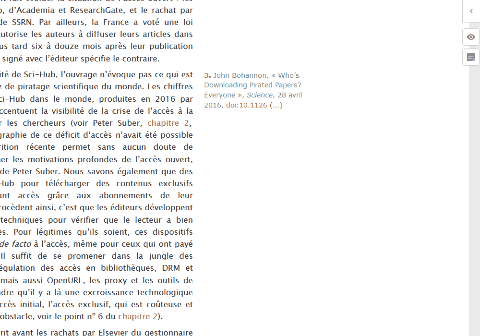
\includegraphics{img/30f5eff1df71626cf0748cd0af596424.png}
\caption{Répondre à une annotation (Source : \href{http://www.maisondesrevues.org/1182}{La maison des revues(2019)})}
\end{figure}

Répondre à une annotation (Source : \href{http://www.maisondesrevues.org/1182}{La maison des revues(2019)})

\hypertarget{s7}{%
\chapter{Exploiter les annotations}\label{s7}}

\hypertarget{s71}{%
\section{Chercher une annotation}\label{s71}}

Ouvrez le document sous hypothesis et cherchez l'annotation. Vous pouvez vous aider de l'outil de recherche (loupe) ou trier les annotations (bouton en forme de double flèche) en haut à droite du volet d'annotation

\begin{figure}
\centering
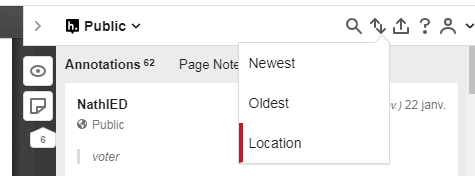
\includegraphics{img/sort.png}
\caption{Rechercher et trier les annotations}
\end{figure}

\hypertarget{tableau-de-bord}{%
\section{Tableau de bord}\label{tableau-de-bord}}

Chaque utilisateur dispose d'un tableau de bord dans lequel il peut retrouver les documents et les annotations qu'il a réalisé ou ceux de ses groupes. Pour ouvrir votre tableau de bord, cliquez sur l'icone de l'utilisateur en haut à droite du volet d'annotation et sélectionnez votre nom.

\begin{figure}
\centering
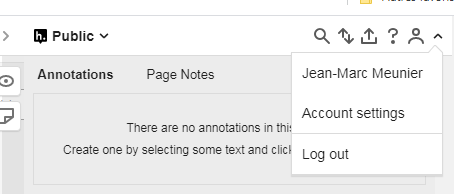
\includegraphics{img/login.png}
\caption{Consulter le tableau de bord}
\end{figure}

Une barre de recherche vous permettra d'explorer vos documents. le tableau de bord donne également la liste de documents que vous avez annoté ainsi qu'un lien vers chacun de ceux-ci. Vous y trouverez également la liste des mots-clés utilisés. En cliquant dessus, vous pouvez filtrer les documents concernés.

\begin{figure}
\centering
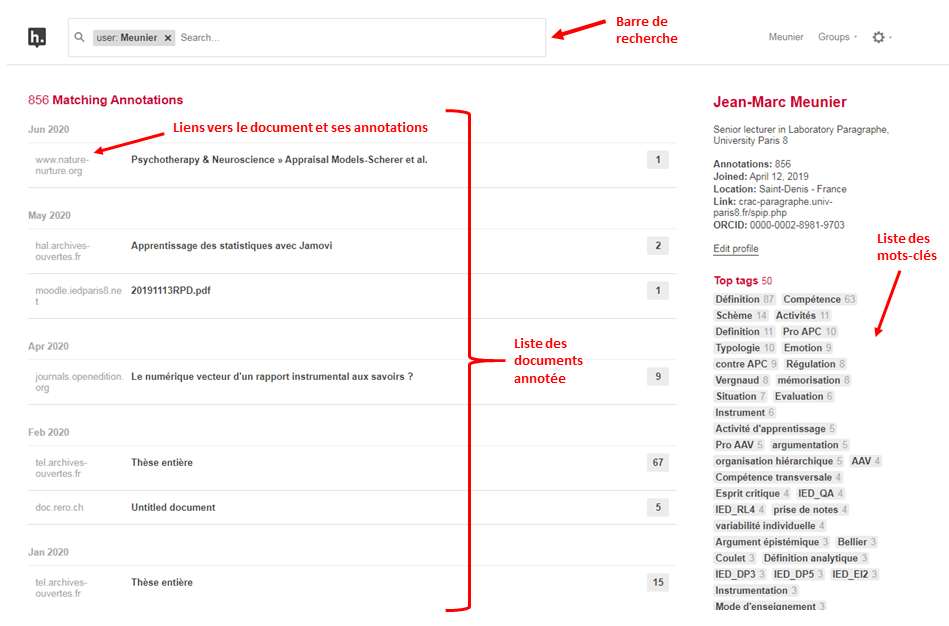
\includegraphics{img/dashboard.png}
\caption{Le tableau de bord}
\end{figure}

Hypothesis offre également la possibilité d'explorer les annotations publiques en allant sur la page dédiée \url{https://hypothes.is/search}

\hypertarget{ruxe9fuxe9rences}{%
\chapter*{Références}\label{ruxe9fuxe9rences}}
\addcontentsline{toc}{chapter}{Références}

La maison des revues (2019). «\,Hypothes.is\,: Guide utilisateur Se repérer\,». La maison des revues. Site d'information et d'accompagnement éditorial. \url{http://www.maisondesrevues.org/1182}

  \bibliography{book.bib,packages.bib}

\end{document}
